\documentclass{beamer}
\usepackage{graphicx} % Images
\usepackage{pgfpages} % Notes for slides
\usepackage{marvosym} % Audio playback symbols
\usepackage{tipa} % IPA phonetic symbols
\usepackage{amsmath} % Math symbols
\usepackage{amssymb} % Math symbols
\usepackage{tikz} % Graphs and plots
\usepackage{booktabs} % Nice tables

\usetheme[dept=ai, coloredtitles, coloredblocks]{vub}
%\setbeameroption{show notes on second screen}

\begin{document}

\title{Advances in the Analysis of \\ Discrete Resonance Spectrograms}
\subtitle{Using the DSR for Source Separation and Sequential Prediction}
\author{Nick Harley \& Steve Homer}
\institute{Vrije Universiteit Brussel}
\date{}
\frame{\titlepage}

%
\begin{frame}
  \frametitle{Two Stacked Blocks}
  \begin{block}{Upper Block with bullets}
    \begin{itemize}
      \item First point \textbf{using emphasis}
      \item Second point \textit{using italics}
      \item Third point \underline{using underline}
    \end{itemize}
  \end{block}
  \begin{block}{Lower Block with numbers}
    \begin{enumerate}
      \item First point \textbf{using emphasis}
      \item Second point \textit{using italics}
      \item Third point \underline{using underline}
    \end{enumerate}
  \end{block}
\end{frame}
\note[enumerate]{
  \item Talking point 1
  \item Talking point 2
  \item Talking point 3
}

\begin{frame}
  \frametitle{Single Block with Headings}
  \begin{block}{Object Detection and Recognition}
    \textbf{First Heading}
    \begin{itemize}
      \item First content
      \item Second content
    \end{itemize}
    \textbf{Second Heading}
    \begin{itemize}
      \item First content
      \item Second content
    \end{itemize}
    \textbf{Third Heading}
    \begin{itemize}
      \item First content
      \item Second content
    \end{itemize}
  \end{block}
\end{frame}
\note[enumerate]{
  \item Talking point 1
  \item Talking point 2
  \item Talking point 3
}

\begin{frame}
  \frametitle{Two Column Blocks}
  \begin{columns}
    \begin{column}{0.5\textwidth}
      \begin{block}{First Column}
        
\includegraphics[width=\textwidth]{images/test.pdf}
      \end{block}
    \end{column}
    \begin{column}{0.5\textwidth}
      \begin{block}{Second Column}
        
\includegraphics[width=\textwidth]{images/test.pdf}
      \end{block}
    \end{column}
  \end{columns}
  \vfill
  \textbf{Flush left} \hfill \textbf{Flush right} \\
  Flush left \hfill Flush right
\end{frame}
\note[enumerate]{
  \item Talking point 1
  \item Talking point 2
  \item Talking point 3
}

\begin{frame}
\frametitle{The Discrete Resonance Spectrogram (DRS)}
	\begin{block}{Overview}
		\begin{itemize}
			\item High resolution spectral analysis of audio signals
			\item Gives precise shape and location of spectral peaks 
			\item Provides access to the content of audio signals
		\end{itemize}
	\end{block}
	\centering
	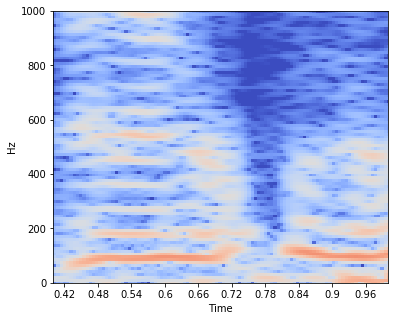
\includegraphics[width=0.45\textwidth]{images/voice-ffts.png}	
	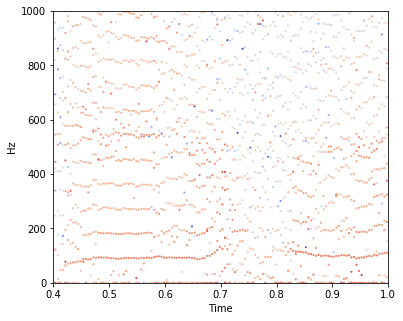
\includegraphics[width=0.45\textwidth]{images/voice-drs.png}	
\end{frame}

\begin{frame}
\frametitle{DRS Advantages and Applications}
	\begin{block}{Target Applications}
		\begin{itemize}
			\item Analysis of voice signals in industrial environments
			\item Vocal signature modelling
			\item Data compression
		\end{itemize}	
	\end{block}
	\begin{block}{Advantages of the DRS}
		\begin{itemize}
			\item Better resolution than FFT based methods
			\item Affords intelligent top-down signal processing
			\item Better integration with symbolic knowledge representation
		\end{itemize}
	\end{block}
\end{frame}

\begin{frame}
\frametitle{Current Objectives}
	\begin{block}{Intelligent bottom-up pattern detection}
		\begin{itemize}
			\item Parameter selection $\checkmark$
			\item Improve time resolution $\checkmark$
			\item Fundamental frequency (F0) tracking $\checkmark$
			\item Source detection and isolation
			\item Noise reduction
		\end{itemize}
	\end{block}
\end{frame}

\begin{frame}
\frametitle{Work to date}
	\begin{columns}
		\begin{column}{0.5\textwidth}
			\begin{block}{Parameter selection \checkmark}	
				An algorithm for automatically selecting parameters, reducing the need for tuning.
			\end{block}
			\begin{block}{Improved time resolution \checkmark}
				A segmentation algorithm which uses smooth sliding window envelopes.
			\end{block}
			\begin{block}{F0 estimation \checkmark}
				An algorithm for tracking fundamental pitch (Geraint).
			\end{block}
		\end{column}
		\begin{column}{0.5\textwidth}
			\begin{tabular}{r l}
				Original signal & $\rhd$ \\
				Basic analysis & $\rhd$  \\ 
				Enhanced analysis & $\rhd$ \\
				& \\
			\end{tabular} 
			\par \scriptsize{F0 tracking works well for simple harmonic sounds such as a flute.} 
			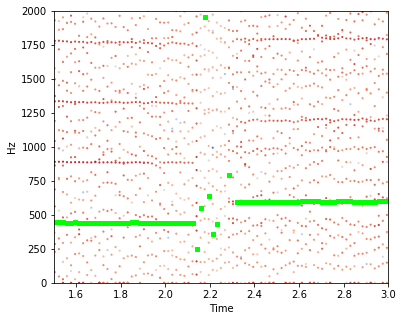
\includegraphics[width=\textwidth]{images/f0-flute.png}
		\end{column}
	\end{columns}			
\end{frame}

\begin{frame}
\frametitle{Immediate Next Steps}
	\begin{columns}
		\begin{column}{0.5\textwidth}
			\begin{block}{Phase and decay}	
				Improve F0 tracking using phase and decay information
			\end{block}
			\begin{block}{Inter-slice information}
				Use previous slice to inform analysis. 
			\end{block}
			\begin{block}{Source isolation}
				Use F0 information to detect and isolate individual sources.
			\end{block}
		\end{column}
		\begin{column}{0.5\textwidth}
			\scriptsize{F0 tracking deteriorates for more complex sounds such as a voice.} 
			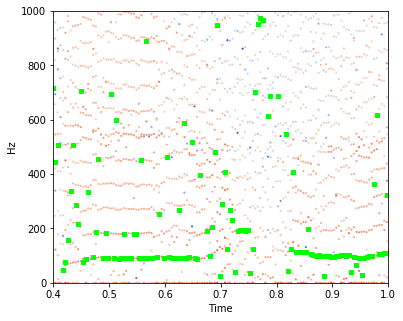
\includegraphics[width=\textwidth]{images/f0-voice.png}
		\end{column}
	\end{columns}			
\end{frame}
\begin{frame}
  \frametitle{Source Separation to Sequential Prediction}
  \begin{block}{Discrete Resonance Spectrogram}
    \textbf{TODO}: (Insert wide aspect ratio image of DRS)
  \end{block}
  \begin{block}{From Vertical to Horizontal Analysis}
    \begin{itemize}
      \item Source separation looks at dependencies between frequencies \textbf{within a slice}, i.e. vertical analysis.
      \item Temporal correlations can be exploited to observe dependencies \textbf{between slices}, i.e. horizontal analysis.
    \end{itemize}
  \end{block}
\end{frame}

\begin{frame}
  \frametitle{Boundary Entropy Segmentation}
\end{frame}

\begin{frame}
  \frametitle{Sequence Interpretation of BES}
\end{frame}

\begin{frame}
  \frametitle{Network Interpretation of BES}
\end{frame}

\begin{frame}
  \frametitle{Hierarchical Structure and Dynamics}
\end{frame}

\begin{frame}
  \frametitle{Minimum Description Length Principle}
\end{frame}

\begin{frame}
  \frametitle{Placement and Next Steps}
  \begin{block}{Placement}
    \begin{itemize}
      \item 
      \item 
      \item 
    \end{itemize}
  \end{block}
  \begin{block}{Next Steps}
    \begin{itemize}
      \item 
      \item
      \item
    \end{itemize}
  \end{block}
\end{frame}

\begin{frame}
  \frametitle{Applications and Future Work}
  \begin{block}{Applications}
    \begin{itemize}
      \item 
      \item 
      \item 
    \end{itemize}
  \end{block}
  \begin{block}{Future Work}
    \begin{itemize}
      \item 
      \item
      \item
    \end{itemize}
  \end{block}
\end{frame}


\begin{frame}
  \frametitle{Thank you!}
  
\includegraphics[width=\textwidth]{dept/vub-ai.pdf}
  \begin{center}
    \huge{Computational Creativity Lab}
  \end{center}
\end{frame}

\end{document}
